\documentclass[12pt]{exam}
\usepackage[margin=0.5in]{geometry}
\usepackage{amsmath,amssymb}
\usepackage{tikz}
\usetikzlibrary{arrows,automata,positioning,trees}
\usepackage{soul}

\newcommand{\blank}[1]{\underline{\hspace*{#1}}}
\newcommand{\ds}{\displaystyle}
\newcommand{\on}{\operatorname}
\newcommand{\mymod}{~\mathrm{mod}~}
\newcommand{\N}{\mathbb{N}}


\begin{document}
\pagestyle{empty}
\graphicspath{{/home/brian/Dropbox/HSC/Spring16/Math111/}}

\subsubsection*{COMS 461 - Midterm 2 Review}

\begin{questions}

\question Create a context free grammar that generates the following language.
$$L = \{ w \in \{a,b\}^* : w \text{ starts and ends with different symbols}\}.$$
\begin{solution}
\begin{align*}
S &\rightarrow aXb ~ | ~ bXa \\
X &\rightarrow aX ~ | ~ bX ~ | ~ \epsilon
\end{align*}
\end{solution}
\vfill
\vfill

\vfill
\question Draw a state diagram for a nondeterministic pushdown automata (NPDA) that recognizes
$$L = \{ w \in \{a,b\}^* : w \text{ starts and ends with different symbols}\}.$$
\begin{solution}
\begin{center}
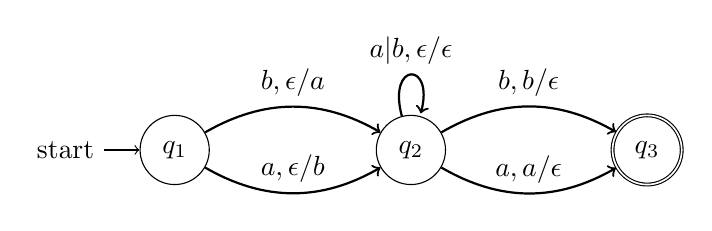
\begin{tikzpicture}[node distance=3cm,auto]
  \node[state,initial]   (q_1)                 {$q_1$};
  \node[state]           (q_2) [right of=q_1]  {$q_2$};
  \node[state,accepting] (q_3) [right of=q_2]  {$q_3$};
  \path[thick,->]
  (q_1) edge [bend right] node {$a, \epsilon/ b$} (q_2)
  (q_1) edge [bend left] node {$b, \epsilon/ a$} (q_2)
  (q_2) edge [loop above] node {$a|b,\epsilon/ \epsilon$} ()
  (q_2) edge [bend right] node {$a, a/ \epsilon$} (q_3)
  (q_2) edge [bend left] node {$b, b/ \epsilon$} (q_3);
\end{tikzpicture}
\end{center}
\end{solution}
\vfill
\vfill


\question Consider the Turing machine with state diagram shown below. 
\begin{center}
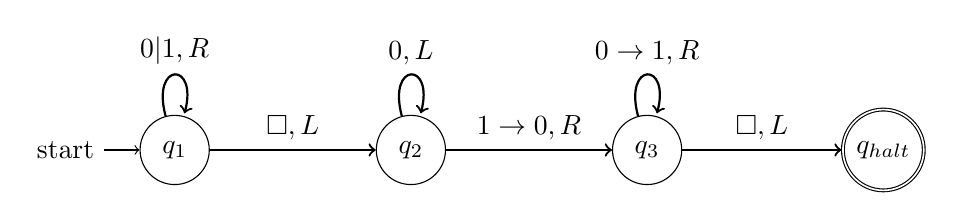
\begin{tikzpicture}[node distance=3cm,auto]
  \node[state,initial]   (q_1)                 {$q_1$};
  \node[state]           (q_2) [right of=q_1]  {$q_2$};
  \node[state]           (q_3) [right of=q_2]  {$q_3$};
  \node[state,accepting] (q_4) [right of=q_3]  {$q_{halt}$};
  \path[thick,->]
  (q_1) edge [loop above] node {$0|1,R$} (q_1)
  (q_1) edge              node {$\square,L$} (q_2)
  (q_2) edge              node {$1 \rightarrow 0,R$} (q_3)
  (q_2) edge [loop above] node {$0, L$} ()
  (q_3) edge [loop above] node {$0\rightarrow 1, R$} ()
  (q_3) edge              node {$\square, L$} (q_4);
\end{tikzpicture}
\end{center}
\begin{parts}
\part What will this TM output if the input tape initially contains the string \verb|101000| and the head is initially pointing at the left-most digit? For your answer, write down the final tape contents and indicate the position of the head when the TM halts.  
\begin{solution}
The tape contains \verb|100111| with head pointed at the rightmost 1.  
\end{solution}
\vfill
\part This TM corresponds to a simple function on binary numbers.  What is that function?  
\begin{solution}
Binary decrement by 1 function.
\end{solution}
\vfill
\end{parts}

\newpage
\question Consider the context free grammar below. 
\begin{align*} 
S &\rightarrow aB ~|~ bA \\
A &\rightarrow a ~|~ aS ~|~ AAB \\
B &\rightarrow b ~|~ bS ~|~ BBA
\end{align*}
This grammar generates the language of all strings in $\{a,b\}^*$ with an equal number of $a$'s and $b$'s. Prove that this grammar is ambiguous by finding two different derivations of the string $abba$.  Draw parse trees for the two different derivations that makes it clear that they are different.  
\begin{solution}
\begin{center}
\begin{tikzpicture}
\begin{scope}[scale=0.6]
    \node {S}
        child { node {a} }
        child { node {B} 
            child { node {b} }
            child { node {S} 
                child { node {b} }
                child { node {A} 
                    child { node {a} }
                }
            }
        };
\end{scope}
\begin{scope}[scale=0.6,xshift = 3in]
    \node {S}
        child { node {a} }
        child { node {B} 
            child { node {B} 
                child { node {b} }
            }
            child { node {B} 
                child { node {b} }
            }
            child { node {A} 
                child { node {a} }
            }
        };
\end{scope}
\end{tikzpicture}
\end{center} 
\end{solution}
\vfill
\vfill

\question The following statements are all false.  For each one, explain why it is false.  
\begin{parts}
\part The is an uncountable number of Turing machines that can be defined with a given input alphabet $\Sigma$ and tape alphabet $\Gamma$.
\begin{solution}
The number of Turing machines is countable, since for every number of states $|Q|$, there is only a finite number of transition functions 
$$\delta: Q \times \Gamma \rightarrow Q \times \Gamma \times \{L, R \}$$
\end{solution}
\vfill
\part For any function $f: \{0,1\}^* \rightarrow \{0,1\}$, you can always find a Turing machine that accepts a string $ w \in \{0,1\}^*$ if and only if $f(w) = 1$, but the Turing machine might loop forever on $w$ if $f(w) = 0$.   
\begin{solution}
Let $L = \{w \in \{0,1\}^* : f(w) = 1 \}$.  Then $L$ is a language which might not be Turing computable.  If it is not Turing computable, then there won't be any Turing machine that accepts it, let alone decides it. 
\end{solution}
\vfill


\part All Turing decidable languages are regular.
\begin{solution}
There are lots of examples of Turing decidable languages that are not regular.  Here is one:
$$L = \{a^n b^n : n \in \N \}.$$
It's very easy to make a TM that decides this language, but it is not regular by the pumping lemma.  
\end{solution}
\vfill

%
%
%\vfill
%
%\part Let $P = \{\langle M \rangle : M \text{ is a Turing machine with only one state}\}$.  Then Rice's theorem implies that $P$ is an undecidable language because both $P$ and its complement $\overline{P}$ (in the language of all TM encodings) are nonempty sets. 
%\begin{solution}
%Rice's theorem does not apply since there are TM's $M_1$ and $M_2$ that accept the same language, but $M_1$ has only one state while $M_2$ has two. 
%\end{solution}
%\vfill
%
%\part No Turing machine $M$ can ever accept its own encoding $\langle M \rangle$. 
%\begin{solution}
%If $M$ is a TM that accepts all strings, then $M$ will accept $\langle M \rangle$.
%\end{solution}
%\vfill

\end{parts}


\newpage
%\question[12] Let 
%$$\text{FINITE} = \{\langle M \rangle : M \text{ is a TM and the set of strings accepted by } M \text{ is finite}\}.$$ 
%Explain clearly why FINITE is an undecidable language. 
%\vfill

\question Let 
$$L_1 = \{a^n \, b \, a^m \, b \, a^n \, : \, m, n \in \N\}$$
and let 
$$L_2 = \{a^n \, b \, a^n \, b \, a^n \,:\, n \in \N \}.$$
\begin{parts}
\part Prove that $L_1$ is context free.
\begin{solution}
The following CFG generates $L_1$:
\begin{align*} 
S &\rightarrow aSa ~|~ B  \\
B &\rightarrow bAb  \\
A &\rightarrow aA ~|~ \epsilon 
\end{align*} 
\end{solution}
\vfill

\part Use the pumping lemma to show that $L_2$ is not context free.  
\begin{solution}
Suppose that $L_2$ is context free.  Then it has a pumping length $p$, and any string in $L_2$ with more than $p$ symbols contains substrings $wxy$ such that at least one of $w$ and $y$ is not empty, $|wxy| \le p$, and $w$ and $y$ can be pumped.  Consider the string $s = a^p b a^p b a^p \in L_2$. 
%Notice that $s$ contains three $a$-portions of length $p$ that are separated by $b$'s. 
Since every string in $L_2$ contains exactly two $b$'s, we know that neither of the pumping substrings $w$ and $y$ can contain a $b$. Also, since the length of $wxy$ is at most $p$, it can only contain $a$'s from at most two of the three $a^p$ substrings. Therefore, if you try to pump $w$ and $y$, the three $a$-portions of the string separated by the $b$'s will no longer have the same length, which contradicts the pumping lemma for context-free languages.  So we conclude that $L_2$ is not context-free. $\square$
\end{solution}
\vfill

\end{parts}

\question Describe a Turing machine that accepts the language 
$$L = \{w \in \{a, b\}^* : w \text{ has a different number of a's and b's} \}.$$
Hint: Use a 2-tape Turing machine.
\begin{solution}
Here is one way to do it. Let the first tape store the input $w$ and the second tape has a single $\#$ symbol at the start position. We'll read $w$ from left to right.
\begin{description}
\item[Step 1.] Read the first character of $w$, if it is $a$, move one space to the right on tape 2 and if it is a $b$, then move one space to the left on tape 2. 
\item[Step 2.] Repeat until you reach a blank on tape 1.  Then accept $w$ if the current position on tape 2 is not $\#$, otherwise reject. 
\end{description}
\end{solution}
\vfill

\end{questions}

\end{document}
